\chapter{\gls{sap}-Prozessanalyse}\label{ch:sap-prozessanalyse}


\section{Der \gls{o2c}-Referenzprozess in \gls{sap} \gls{s/4hana}}\label{sec:o2c-referenzprozess}

\gls{sap} bildet den \gls{o2c}-Prozess im Modul \gls{sd} als durchgängige Belegkette ab. Auf ein Angebot folgt der Terminauftrag, daraus wird die Auslieferung erzeugt, nach Kommissionierung und Warenausgangsbuchung entsteht die Faktura, die automatisch einen Buchhaltungsbeleg in der Finanzbuchhaltung erzeugt (Abbildung~\ref{fig:sap-belegfluss}) \parencites[Folie~62 f.]{coletta2026_0303}[S.~63 ff.]{scheibler2021vertrieb}. \gls{erp}-Software ist dabei Standardsoftware mit vordefinierten Geschäftsprozessen, die sich an Best Practices orientieren und per Parametrisierung (Customizing) angepasst werden \parencite[Folie~41]{coletta2026_0303}. Dieser Referenzprozess dient in Kapitel~\ref{ch:fitgap} als Soll-Modell und ist die Vorlage des synthetischen Logs aus Kapitel~\ref{sec:datengrundlage}. Die Belegkette ist dabei nicht nur betriebswirtschaftlich, sondern datentechnisch bedeutsam, denn jeder Übergang zwischen zwei Belegen wird in der Belegflusstabelle festgehalten und lässt sich später als Prozesskante rekonstruieren. Der Soll-Ablauf gibt damit zugleich vor, welche Aktivitäten und Übergänge im Event-Log überhaupt erwartet werden.

Dass die Auftragsabwicklung ein maßgebender Anwendungsfall ist, zeigt das eigene \gls{sap}-Produktangebot. \gls{papm} liefert einen vorkonfigurierten Beispielinhalt „Process Mining on \gls{sap} \gls{s/4hana}“, der die Auftragsabwicklung als eigenes Szenario abbildet und Beispielprozessdaten aus \gls{sap}-Standardtabellen entlang der Schritte Dateneingabe und -prüfung, Verarbeitung und Reporting auswertet. Als integrierte Datenquellen nutzt dieses Modell exakt die Beleg-, Belegfluss- und Änderungsbelegtabellen, die auch Tabelle~\ref{tab:zentrale-sap-tabellen} dieser Arbeit ausweist, ergänzt um den Kundenstamm (KNA1) und die Anmeldedaten (\gls{usr02}) \parencite[Abschnitt~2.1 und 3.1, S.~9--18]{sap2022samplecontent}. Die hier genutzte Werkzeugkette bildet damit methodisch nach, was \gls{sap} für dasselbe Prozessfeld bereits produktiv unterstützt.

\begin{figure}[!htb]
\centering
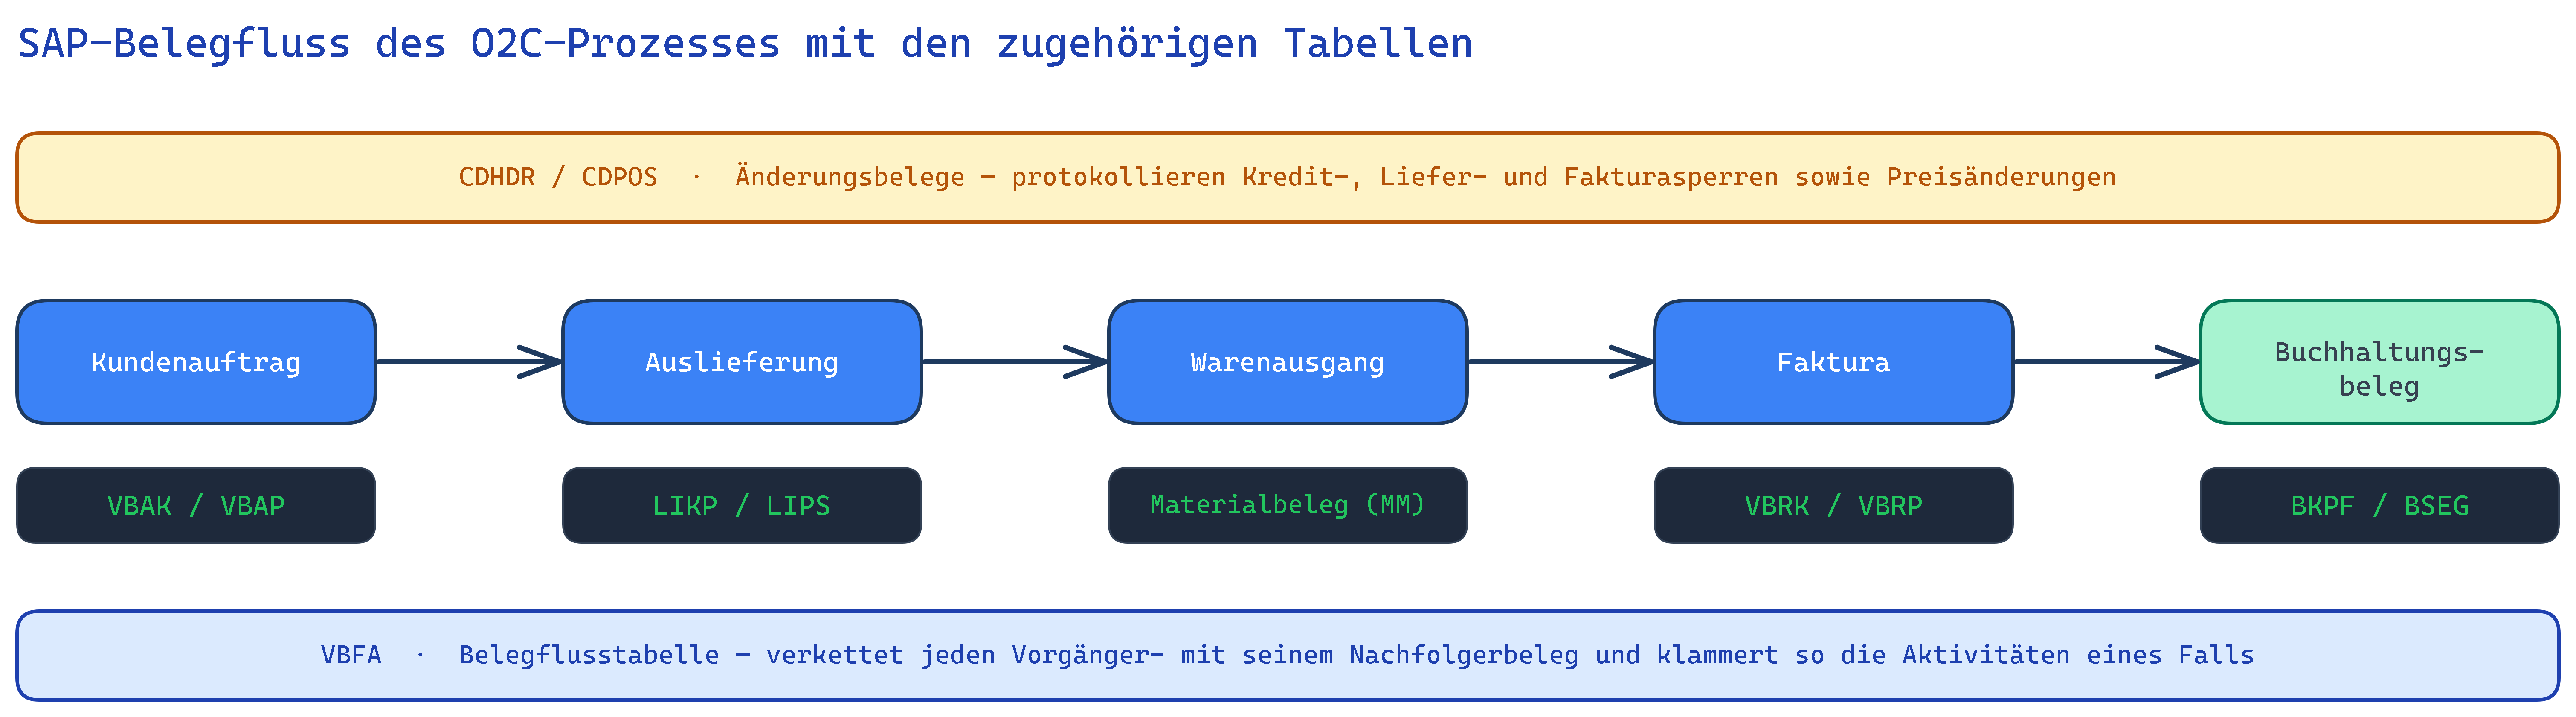
\includegraphics[width=\textwidth,height=0.36\textheight,keepaspectratio]{figures/image2.png}
\caption{\gls{sap}-Belegfluss des \gls{o2c}-Prozesses mit den zugehörigen Tabellen (Quelle: eigene Darstellung)}\label{fig:sap-belegfluss}
\end{figure}

Der eigentliche Prozess ist reicher als die reine Soll-Kette, denn an mehreren Stellen sieht der Standard Prüfungen und mögliche Sperren vor: Die Kreditprüfung kann einen Auftrag sperren, bis er freigegeben wird, die Unvollständigkeits- und Verfügbarkeitsprüfung kann die Lieferung verzögern, und Preisabweichungen können eine Fakturasperre auslösen. Ob diese Prüfungen automatisiert oder manuell, streng oder locker eingestellt sind, ist eine Frage des Customizings und damit genau der Stellhebel, an dem die Verbesserungsmaßnahmen in Kapitel~\ref{ch:anpassung} ansetzen. Ergänzend trägt jeder Beleg einen Belegtyp und einen Status (Gesamtbearbeitungs-, Liefer-, Warenausgangs- und Fakturastatus): Der Belegtyp bestimmt die zulässigen Folgebelege, der Status dokumentiert den Fortschritt und ist damit eine zum Belegfluss komplementäre Ereignisquelle für das Process Mining.

\section{Stamm- und Bewegungsdaten im \gls{sap}-Prozess}\label{sec:stamm-bewegungsdaten-sap}

\gls{sap} bildet ein Unternehmen über eine Hierarchie von Organisationseinheiten ab. An der Spitze steht der Mandant als betriebswirtschaftlich größte organisatorische Einheit, darunter der Buchungskreis als kleinste Einheit, für die eine vollständige, in sich abgeschlossene Buchhaltung geführt werden kann \parencites[Folien~357 ff.]{coletta2026_0206}[Folien~484 ff.]{coletta2026_1407}. Organisatorisch wird der Vertrieb über die Einheiten Verkaufsorganisation, Vertriebsweg und Sparte strukturiert, die zusammen den Vertriebsbereich bilden. Die Versandstelle bündelt die Versandaktivitäten für ein oder mehrere Werke \parencites[Folie~492, 520 f.]{coletta2026_1407}[Folie~398]{coletta2026_0906}. Diese Organisationsdaten sind für Process Mining nicht nur Kontext, sondern ein wertvolles Filterkriterium, weil sie den Vergleich von Prozessvarianten je Verkaufsorganisation oder Versandstelle erlauben. Der Kundenstamm wird in \gls{s/4hana} als Geschäftspartner geführt und gliedert sich in mandantenweite allgemeine Daten, Buchungskreisdaten der Finanzbuchhaltung und Vertriebsbereichsdaten \parencite[Folie~492, 502, 520 f.]{coletta2026_1407}. Der Materialstamm ist die „zentrale Quelle zum Abruf materialspezifischer Daten“ und in funktionale Sichten gegliedert \parencite[Folie~499 ff.]{coletta2026_1407}. Gerade die Vertriebsbereichsdaten des Kundenstamms, etwa Versandbedingungen und Incoterms, sind es, deren Lückenhaftigkeit im Ist-Prozess die Liefersperren (K3) auslöst. Ähnlich verhält es sich mit dem Konditionsstamm: Sind Sonderpreise dort nicht hinterlegt, weichen die Sachbearbeiter auf manuelle Eingaben im Auftrag aus, was die Fakturasperren (K5) nach sich zieht. Die Qualität der Stammdaten bestimmt somit unmittelbar, wie viele Fälle den störungsfreien Pfad verlassen, und ist damit der zentrale Ansatzpunkt jeder nachhaltigen Verbesserung.

Die Bewegungsdaten liegen in relationalen Tabellenpaaren aus Kopf- und Positionsdaten (Tabelle~\ref{tab:zentrale-sap-tabellen}). Drei Eigenschaften sind für die vorliegende Fragestellung entscheidend. Erstens trägt jeder Beleg Zeitstempel und Benutzerkennung (z.\,B. \gls{erdat}/\gls{erzet}/\gls{ernam}), sodass Ereigniszeitpunkte rekonstruierbar sind. Zweitens dokumentiert die Belegflusstabelle \gls{vbfa} jede Vorgänger-Nachfolger-Beziehung zwischen Belegen und verknüpft damit die Prozessschritte eines Falls. Drittens protokollieren Änderungsbelege (\gls{cdhdr}/\gls{cdpos}) jede nachträgliche Änderung an Belegen und Stammdaten einschließlich Datum, Uhrzeit, Benutzer und geändertem Feld. Über sie werden auch das Setzen und Lösen von Kredit-, Liefer- und Fakturasperren sichtbar \parencites[S.~63 ff.]{scheibler2021vertrieb}[Folie~375]{coletta2026_0206}. Technisch liegen alle genannten Tabellen in \gls{s/4hana} auf der spaltenorientierten In-Memory-Datenbank \gls{sap} HANA, was Massenauswertungen direkt auf den Bewegungsdaten beschleunigt \parencite[Folie~266]{coletta2026_1905}. Besonders die Änderungsbelege sind für die vorliegende Fragestellung wertvoll, weil sie Zustandsübergänge festhalten, die in den reinen Belegtabellen unsichtbar blieben: Ob und wann eine Kreditsperre gesetzt und wieder gelöst wurde, ergibt sich erst aus der Historie des Feldes \gls{cmgst} in \gls{cdpos}. Ohne diese Protokollierung wären die Sperrenmuster K2, K3 und K5 aus den Daten nicht rekonstruierbar; sie sind der Grund, warum ein Event-Log deutlich mehr Aktivitäten enthalten kann als der reine Belegfluss nahelegt.

\begin{table}[!htb]
\centering
\caption{Zentrale \gls{sap}-Tabellen des \gls{o2c}-Prozesses (Auswahl)}\label{tab:zentrale-sap-tabellen}
\small
\begin{tabularx}{\textwidth}{@{}>{\RaggedRight\arraybackslash}p{2.5cm} >{\RaggedRight\arraybackslash}p{4.4cm} Y@{}}
\toprule
\textbf{Beleg /\allowbreak{} Objekt} & \textbf{Kopf-/\allowbreak{}Positionstabelle} & \textbf{Für Process Mining relevante Felder} \\
\midrule
Kundenauftrag & \gls{vbak} /\allowbreak{} \gls{vbap} & VBELN, POSNR, \gls{erdat}/\allowbreak{}\gls{erzet}/\allowbreak{}\gls{ernam}, AUART, NETWR, \gls{lifsk}, \gls{cmgst} \\
Auslieferung & \gls{likp} /\allowbreak{} \gls{lips} & VBELN, \gls{erdat}/\allowbreak{}\gls{erzet}, \gls{lfdat}, WADAT\_IST (tatsächl. Warenausgang) \\
Faktura & \gls{vbrk} /\allowbreak{} \gls{vbrp} & VBELN, \gls{erdat}/\allowbreak{}\gls{erzet}, FKDAT, \gls{fksto}, NETWR \\
Buchhaltungsbeleg & \gls{bkpf} /\allowbreak{} \gls{bseg} (ACDOCA) & BELNR, BUDAT, \gls{augdt} \\
Belegfluss & \gls{vbfa} & VBELV/\allowbreak{}POSNV $\rightarrow$ VBELN/\allowbreak{}POSNN, VBTYP\_N, \gls{erdat}/\allowbreak{}\gls{erzet} \\
Änderungsbelege & \gls{cdhdr} /\allowbreak{} \gls{cdpos} & OBJECTCLAS (z. B. VERKBELEG), UDATE/\allowbreak{}UTIME, USERNAME, TABNAME, FNAME, Alt-/\allowbreak{}Neuwert \\
\bottomrule
\end{tabularx}
\end{table}


\section{Schnittpunkte mit anderen \gls{sap}-Modulen}\label{sec:modulschnittstellen}

Der \gls{o2c}-Prozess ist kein reiner \gls{sd}-Prozess, sondern lebt von der Integration (Tabelle~\ref{tab:modulschnittstellen}). Die Verfügbarkeitsprüfung und die Warenausgangsbuchung greifen auf die Bestandsführung des Moduls \gls{mm} zu, kundenauftragsbezogene Fertigungsaufträge entstehen im Modul \gls{pp}, die Faktura erzeugt den Buchhaltungsbeleg und den offenen Posten in \gls{fi}, das Kreditmanagement bewertet den Debitor aus \gls{fi}-Daten, und die Ergebnisrechnung im \gls{co} übernimmt Erlöse und Kosten je Marktsegment.

\begin{table}[!htb]
\centering
\caption{Schnittstellen des \gls{o2c}-Prozesses zu anderen \gls{sap}-Modulen}\label{tab:modulschnittstellen}
\small
\begin{tabularx}{\textwidth}{@{}>{\RaggedRight\arraybackslash}p{3.6cm} >{\RaggedRight\arraybackslash}p{2.8cm} Y@{}}
\toprule
\textbf{\gls{o2c}-Schritt} & \textbf{beteiligtes Modul} & \textbf{ausgetauschtes Datenobjekt /\allowbreak{} Wirkung} \\
\midrule
Verfügbarkeitsprüfung (ATP) & \gls{mm} (ggf. \gls{pp}) & Bestands-/\allowbreak{}Bedarfsabgleich; bei Fehlbestand Anstoß von Beschaffung oder Fertigung \\
Warenausgang buchen & \gls{mm} /\allowbreak{} \gls{fi} & Materialbeleg mindert Bestand; Buchungsbeleg bucht Warenaufwand \\
Faktura erstellen & \gls{fi} & debitorischer offener Posten (Forderung) wird erzeugt \\
Kreditprüfung & \gls{fi} (\gls{fscm}) & Bewertung des Debitors anhand Kreditlimit und offener Posten \\
Erlös-/Kostenzuordnung & \gls{co} & Übernahme von Erlösen und Kosten in die Ergebnisrechnung \\
\bottomrule
\end{tabularx}
\end{table}

Diese Integration über eine gemeinsame Datenhaltung ist ein Grundprinzip von \gls{erp}-Systemen \parencite[Folie~44 und 63]{coletta2026_0303} und der Grund, warum sich gerade \gls{erp}-Systeme für Process Mining eignen. Weil Informationssilos aufgebrochen und Teilprozesse miteinander verbunden sind \parencite[Folie~74]{coletta2026_1003}, hinterlässt ein Geschäftsfall seine vollständige Spur in einem einzigen System, vom Auftrag bis zum Zahlungseingang. Dass jeder Schritt dabei unmittelbar auf Bestand und Buchhaltung durchschlägt, zeigt \gls{sap} auch in eigenen Schulungsunterlagen, dort am Beispiel von \gls{sap} Business One \parencite[S.~2]{sap2013tb1000}.

Für die Analyse folgt daraus eine praktische Konsequenz: Ein vollständiges Bild des \gls{o2c}-Prozesses erfordert Daten aus mehreren Modulen. Die reinen Vertriebsbelege zeigen den Auftrag und die Rechnung, nicht aber die Bestandsbuchung im \gls{mm} oder den Zahlungsausgleich im \gls{fi}. Erst die modulübergreifende Extraktion, die \gls{sap} über die gemeinsame Datenbank technisch ermöglicht, erlaubt es, den Prozess lückenlos vom Auftrag bis zum Geldeingang abzubilden.
